\section{Fundamentos teóricos}

\begin{frame}{Referencia anatómica}
    \begin{columns}[c,onlytextwidth]
        \begin{column}{0.50\textwidth}
            \centering
            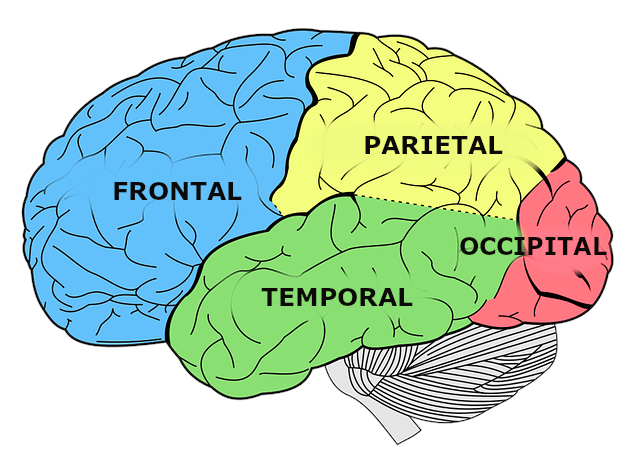
\includegraphics[width=0.92\textwidth]{../memoria/figs/lobulos_cerebrales.png}
        \end{column}

        \begin{column}{0.46\textwidth}
            \begin{tikzpicture}[
                zona/.style={
                    rectangle,
                    rounded corners=3pt,
                    fill=urjcred!8,
                    draw=urjcred!35,
                    text width=4.6cm,
                    minimum height=0.78cm,
                    align=left,
                    font=\small,
                    inner xsep=8pt
                }
            ]
                \node[zona] (a) {\textbf{Frontal}\\pensamiento consciente};
                \node[zona, below=0.28cm of a] (b) {\textbf{Temporal}\\oído, olfato, estímulos complejos};
                \node[zona, below=0.28cm of b] (c) {\textbf{Parietal}\\integración sensorial};
                \node[zona, below=0.28cm of c] (d) {\textbf{Occipital}\\visión};
            \end{tikzpicture}
        \end{column}
    \end{columns}
\end{frame}

\begin{frame}{Bandas espectrales}
    \centering
    \renewcommand{\arraystretch}{1.22}
    \begin{tabular}{lll}
        \toprule
        \textbf{Banda} & \textbf{Rango} & \textbf{Idea clave} \\
        \midrule
        Delta & 1--4 Hz & sueño profundo / baja actividad consciente \\
        Theta & 4--8 Hz & somnolencia / relajación \\
        Alpha & 8--12 Hz & despierto pero tranquilo \\
        Beta & 12--30 Hz & atención / concentración \\
        Gamma & \(>30\) Hz & integración de información \\
        \bottomrule
    \end{tabular}

    \vspace{0.55cm}
    \begin{tikzpicture}[
        bloque/.style={
            rectangle,
            rounded corners=3pt,
            fill=urjcred!8,
            draw=urjcred!35,
            text width=9.5cm,
            align=center,
            minimum height=0.78cm,
            font=\small
        }
    ]
        \node[bloque] {El modelo no recibe ``emociones'' directamente: trabaja con potencia por bandas y canales.};
    \end{tikzpicture}
\end{frame}

\begin{frame}{Topomaps}
    \begin{columns}[c,onlytextwidth]
        \begin{column}{0.47\textwidth}
            \centering
            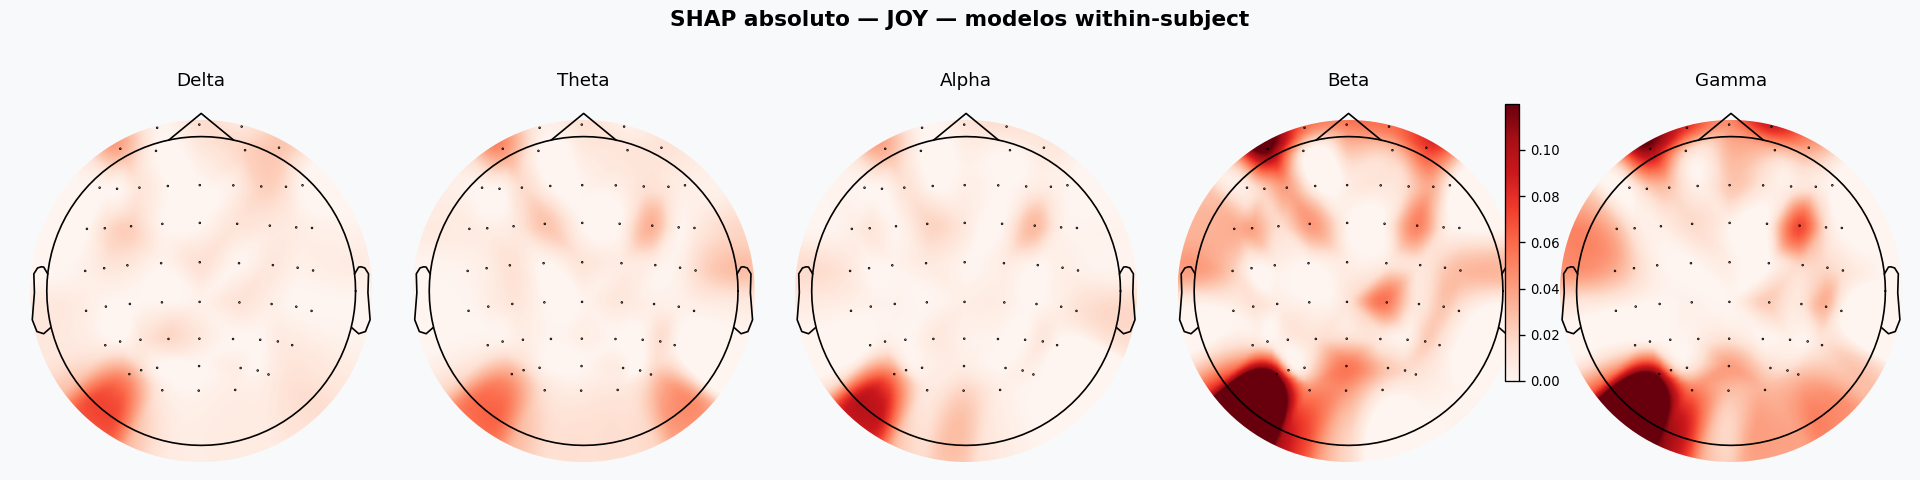
\includegraphics[width=0.86\textwidth]{../memoria/figs/topomap_ejemplo.png}
        \end{column}

        \begin{column}{0.48\textwidth}
            \begin{tikzpicture}[
                idea/.style={
                    rectangle,
                    rounded corners=3pt,
                    fill=softblue!10,
                    draw=softblue!45,
                    text width=5.45cm,
                    minimum height=1.08cm,
                    align=left,
                    font=\small,
                    inner xsep=8pt
                }
            ]
                \node[idea] (a) {\textbf{Electrodos}\\cada posición aporta un valor};
                \node[idea, below=0.34cm of a] (b) {\textbf{Color}\\representa la magnitud o contribución};
                \node[idea, below=0.34cm of b] (c) {\textbf{Mapa}\\resume el patrón espacial del modelo};
            \end{tikzpicture}
        \end{column}
    \end{columns}

    \vspace{0.25cm}
    \begin{center}
        {\scriptsize Un topomap no ``lee'' emociones: ayuda a visualizar qué zonas aportan información.}
    \end{center}
\end{frame}
